\documentclass[preview,convert={outext=.png}]{standalone}

\usepackage{tikz}
\usetikzlibrary{calc,quotes}

\usepackage{xcolor}

\begin{document}
\pagecolor{white}
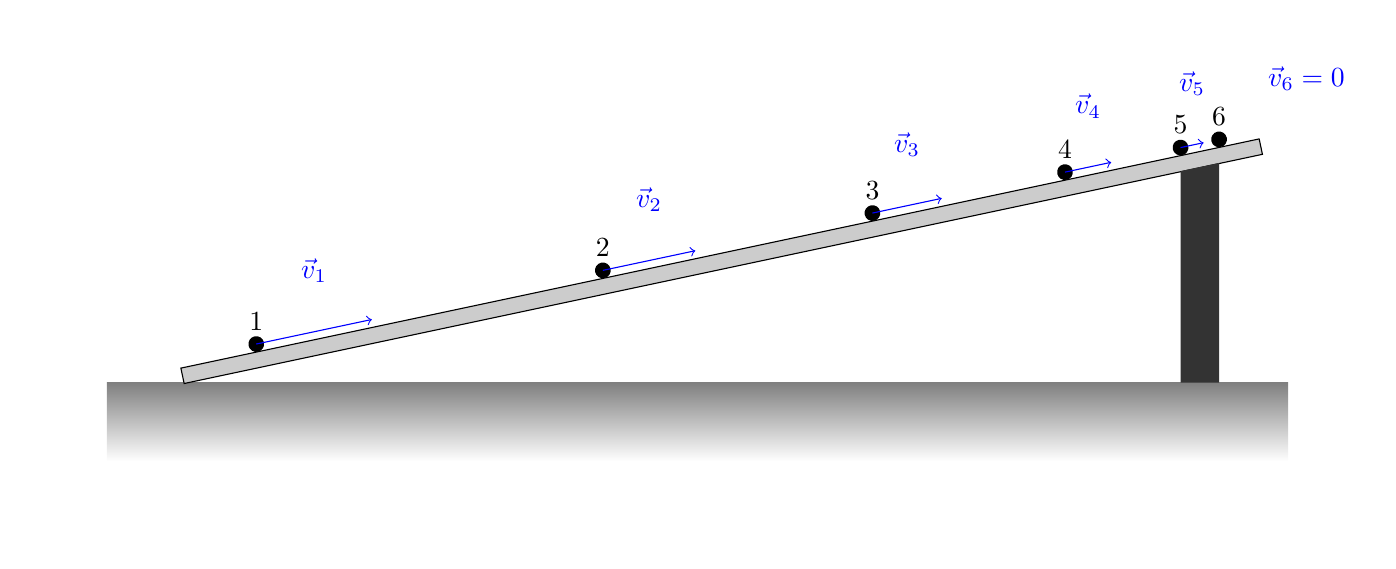
\begin{tikzpicture}
  \draw[white] (-3,-2) rectangle (14,4.5);
  % Make the table top
  \coordinate (O) at (0,0);
  \shade (-2,0) rectangle ++(15,-1);

  % Create the ramp
  \begin{scope}[rotate=12,shift={(0,0.5)}]
    \coordinate (x) at (0,0);
    \coordinate (vi) at (5,0);
    \coordinate (a) at (-1,0);
    \coordinate (v) at (5,0);
    
    \foreach \i in {1,2,3,...,6}{
      \fill (x) circle (0.1) node [above=1.5pt]{\i};

      % Draw the velocity vector, try to make it so it doesn't overlap
      \ifnum \i<6
        \draw[blue, ->] (x) -- ($(x) + 0.3*(v)$) node[midway, above=0.5cm]{$\vec{v}_{\i}$};
      \fi
      \ifnum \i=6
        \node[above right=0.5cm, blue] at (x) {$\vec{v}_{\i}=0$};
      \fi

      % Need this to save the coordinate of the top
      \coordinate (top) at (x);
      % Update the position and velocity vectors
      \coordinate (x) at ($(x) + (v) + 0.5*(a)$);
      \coordinate (v) at ($(v) + (a)$);
    }
    \filldraw[color=black,fill=black!20] (-1,-0.1) rectangle ++(14,-0.2);
  \end{scope}

  %% Draw the "post" holding up the ramp.
  \coordinate (T) at ($(x) - (0,0.3)$);
  \coordinate (S) at ($(top) - (0,0.3)$);
  \fill[black!80] (S) -- (T) -- (O -| T) -- (O -| S) -- cycle;
\end{tikzpicture}
\end{document}